\documentclass[10pt]{article}
\usepackage[polish]{babel}
\usepackage[utf8]{inputenc}
\usepackage[T1]{fontenc}
\usepackage{amsmath}
\usepackage{amsfonts}
\usepackage{amssymb}
\usepackage[version=4]{mhchem}
\usepackage{stmaryrd}
\usepackage{graphicx}
\usepackage[export]{adjustbox}
\graphicspath{ {./images/} }

\title{GIMNAZJUM }

\author{}
\date{}


\begin{document}
\maketitle
\begin{enumerate}
  \item Na globusie w kształcie kuli o promieniu \(R\) zakreślono cyrklem o rozwartości \(R\) okrąg (nóżkę cyrkla umieszczono na biegunie). Jaka jest długość narysowanego równoleżnika?
  \item Punkt \(H\) jest punktem przecięcia wysokości w trójkącie ostrokątnym \(A B C\). Odcinki \(A B\) i \(C H\) mają jednakową długość. Jaka jest miara kąta \(A C B\) ?
  \item Rozwiąż w liczbach całkowitych równanie \(2^{x}(6-x)=8 x\)
\end{enumerate}

\section*{LICEUM}
\begin{enumerate}
  \item Punkt \(M\) jest środkiem boku \(A B\) kwadratu \(A B C D\) o boku długości 1. Oblicz pole zacieniowanego obszaru.
  \item Oblicz wartość iloczynu \(x y z\), wiedząc, że \(x^{2} y z^{3}=7^{3}\) oraz\\
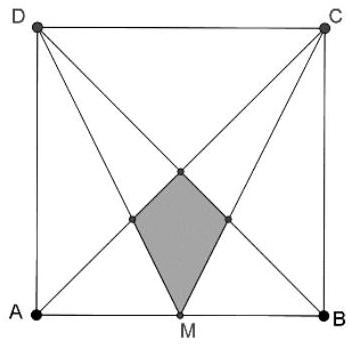
\includegraphics[max width=\textwidth, center]{2024_11_21_22b13a6aca32b5fedbe5g-1}\\
\(x y^{2}=7^{9}\).
  \item Jasiu ma 36 drewnianych klocków. Pomalował je używając trzech kolorów: białego, brązowego i czarnego. Niektóre klocki pomalował tylko jednym kolorem, inne dwoma a pozostałe 5 klocków wszystkimi trzema kolorami. Białej farby użył do pomalowania 25 klocków, brązowej do pomalowania 28 klocków, a czarnej do pomalowania 20 klocków. Ile klocków pomalował tylko jednym kolorem?
\end{enumerate}

\end{document}